\documentclass{beamer}
\usepackage[utf8]{inputenc}
\usepackage{graphicx}
\usepackage{xcolor}
\usepackage{listings}
\usepackage{tikz}

\usetikzlibrary{fit}


\title{Implementation of the TIL-Script Language}
\author{Filip Peterek}
\institute{VSB -- Technical University of Ostrava}
\date{May 2023}

\begin{document}

\frame{\titlepage}

\section{Project Goals}

\begin{frame}
    \frametitle{Project Goals}
    \begin{itemize}
        \item Define the TIL-Script programming language
        \item Create a working TIL-Script interpreter
        \item Document the language properly
    \end{itemize}
\end{frame}

\section{Theoretical Background}

\begin{frame}
    \frametitle{Transparent Intensional Logic}
    \begin{itemize}
        \item Logical analysis of natural language
        \item Based on typed Lambda calculi
        \item Rigorously defined type hierarchy
        \item Procedural and hyperintensional
        \item Constructions can mention other constructions
        \item Sentence meaning is carried by a procedure
            \begin{itemize}
                \item We mostly care for the procedure itself, seldom do we care for the value
                it produces
            \end{itemize}
    \end{itemize}
\end{frame}

\section{TIL-Script}

\begin{frame}
    \frametitle{TIL-Script}
    \begin{itemize}
        \item Grammar closely resembles TIL grammar
        \item Adds upon TIL to form a useable programming language
            \begin{itemize}
                \item Lists
                \item Tuples
                \item Structures
                \item Strings
            \end{itemize}
        \item Also adds restrictions imposed by computers with finite resources
    \end{itemize}
\end{frame}

\begin{frame}
    \frametitle{Original Features}
    \begin{itemize}
        \item Grammar, but no semantics
        \item All TIL constructions
        \item 
    \end{itemize}
\end{frame}

\section{Implementation}

\begin{frame}
    \frametitle{Implementation}
    \begin{itemize}
        \item Kotlin
        \item Gradle
        \item Antlr
    \end{itemize}
\end{frame}

\begin{frame}
    \frametitle{Project Structure}

    \begin{figure}
        \centering
        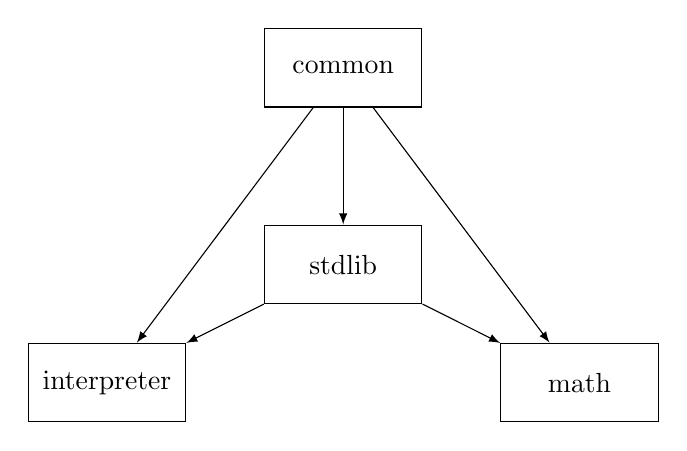
\begin{tikzpicture}
            \node[draw, fit={(0, 0) (2, 1)},                xshift=3cm, inner sep=0pt, label=center:common] (A) {};
            \node[draw, fit={(0, 0) (2, 1)}, yshift=-2.5cm, xshift=3cm, inner sep=0pt, label=center:stdlib] (B) {};

            \node[draw, fit={(0, 0) (2, 1)}, yshift=-4cm,   xshift=6cm, inner sep=0pt, label=center:math] (C) {};
            \node[draw, fit={(0, 0) (2, 1)}, yshift=-4cm,   xshift=0cm, inner sep=0pt, label=center:interpreter] (D) {};

            \draw [-latex]          (A)--(B);
            \draw [-latex]          (A)--(C);
            \draw [-latex]          (A)--(D);
            \draw [-latex]          (B)--(C);
            \draw [-latex]          (B)--(D);
        \end{tikzpicture}
        \caption{Project Structure}
    \end{figure}

\end{frame}

\begin{frame}
    \frametitle{Parser Implementation}
    \begin{itemize}
        \item Existing TIL-Script grammar has been utilized
            \begin{itemize}
                \item Slight tweaks were necessary to make it work with Antlr
            \end{itemize}
        \item Parser is generated using Antlr
        \item Resulting AST is converted to a custom structure
    \end{itemize}
\end{frame}

\begin{frame}
    \begin{center}
        \Huge The End
    \end{center}
\end{frame}

\end{document}
